\documentclass[10pt,twocolumn]{article}

\usepackage[letterpaper,top=0.72in,bottom=0.78in,left=0.70in,right=0.70in]{geometry}
\usepackage[T1]{fontenc}
\usepackage{newtxtext,newtxmath}
\usepackage{microtype}
\usepackage{booktabs}
\usepackage{graphicx}
\usepackage{enumitem}
\usepackage{caption}
\usepackage{xcolor}
\usepackage{natbib}
\usepackage{fancyhdr}
\usepackage{flushend}
\usepackage[hidelinks]{hyperref}

\definecolor{paperblue}{HTML}{1D4ED8}
\definecolor{papergray}{HTML}{4B5563}
\hypersetup{
  colorlinks=true,
  linkcolor=paperblue,
  citecolor=paperblue,
  urlcolor=paperblue,
  pdfauthor={Anonymous Author(s)},
  pdftitle={When Graph Expansion Helps and Hurts}
}

\setlength{\columnsep}{0.24in}
\setlength{\parindent}{1em}
\setlength{\parskip}{0pt}
\setlist{nosep,leftmargin=*}
\captionsetup{font=small,labelfont=bf}
\renewcommand{\arraystretch}{1.08}

\pagestyle{fancy}
\fancyhf{}
\fancyhead[L]{\small\color{papergray}When Graph Expansion Helps and Hurts}
\fancyhead[R]{\small\color{papergray}Anonymous manuscript}
\fancyfoot[C]{\thepage}
\setlength{\headheight}{13pt}

\title{\vspace{-1.5em}\textbf{When Graph Expansion Helps and Hurts}}
\author{Anonymous Author(s)\\
\small Independent Research Manuscript}
\date{}

\begin{document}
\maketitle
\thispagestyle{fancy}

\begin{abstract}
This is a fixed-budget measurement and a partial replication, not a new
retrieval method. On a 141,232-document HotpotQA distractor corpus, all 5,918
validation bridge questions have their two gold paragraphs directly
hyperlinked, against 1 of 1,487 comparison questions, because HotpotQA builds
bridge questions from hyperlinks. 31.5\% of the corpus's 242,196 in-corpus
hyperlinks point into validation gold, which is 9.8\% of the documents. On
this corpus, adding the one-hop hyperlink neighbors of eight hybrid seeds and
reranking with BGE raises complete recall from 0.784 to 0.934 against an
equal-size hybrid pool. The gain is +0.191 on bridge questions and $-0.013$ on
comparison questions. No learned edge scorer is involved. A random-edge control
scores 0.705, but it is weak, because it also falls below its own equal-size
hybrid pool (0.799). On LitSearch, citation expansion hurts overall
($-0.037$ Recall@20, [$-0.068$, $-0.007$]) and on author-written queries, and
helps only inline ACL queries (+0.112). Rescue-coverage and target-degree
diagnostics reuse gold labels or restate one-hop reachability, so they are
descriptive. I did not run a multi-hop retriever baseline.
\end{abstract}

\section{Introduction}

Hybrid retrieval combines lexical precision with semantic matching, but both
arms score documents mainly from their contents. They can miss evidence that is
easy to reach through hyperlinks, citations, or other corpus relations. Prior
work already shows that following Wikipedia hyperlinks improves multi-hop
retrieval on HotpotQA \citep{asai2020paths}, and that corpus-graph neighbors
can improve reranking \citep{macavaney2022gar}. The cluster hypothesis and
score propagation give the older rationale: related documents tend to share
relevance \citep{voorhees1985cluster,diaz2005regularizing}.

Reported gains are hard to attribute. Graph methods change the candidate count,
the scoring budget, and often the reranker at the same time. A gain can come
from a larger pool, a stronger scorer, or the graph itself. Query expansion has
the same problem in another form: it helps some queries and hurts others, which
motivates selective expansion \citep{cronentownsend2004selective}. I ask a
narrow question:

\begin{quote}
Under a fixed candidate budget and a fixed reranker, when does a corpus relation
recover evidence that hybrid retrieval misses, and when does it hurt?
\end{quote}

I evaluate the simplest form of graph expansion: take eight hybrid seeds, add
their one-hop graph neighbors, and rerank that pool with the same
cross-encoder as an equal-size hybrid pool. The research questions are:

\begin{enumerate}[label=\textbf{RQ\arabic*}]
  \item Does the hyperlink pool beat equal-size hybrid, random-edge, and
    dense-feedback pools under the same reranker, and why?
  \item Does extra graph reachability survive reranking?
  \item Does the effect transfer across corpora and query sources?
  \item How do gain and rescue decompose by gold reachability and target
    in-degree?
\end{enumerate}

The contributions are:
\begin{enumerate}
  \item A matched measurement on the HotpotQA distractor corpus, with its
    cause made explicit. One-hop hyperlink pools raise BGE-reranked complete
    recall by 0.150 over equal-size hybrid pools. The gain sits on bridge
    questions, whose gold pairs are hyperlinked by construction.
  \item A negative transfer result on LitSearch. Citation expansion lowers
    overall Recall@20 by 0.037, hurts author-written queries, and helps only
    inline ACL queries under the same reranker.
  \item Two descriptive decompositions, stated with their limits. Rescue
    coverage and gain share gold labels, and the degree contrast is mostly a
    reachability fact.
\end{enumerate}

\section{Related Work}

\paragraph{Hyperlink and multi-hop retrieval.}
\citet{asai2020paths} retrieve reasoning paths over the Wikipedia hyperlink
graph. On the HotpotQA full-wiki setting, adding hyperlinked paragraphs to the
top 20 TF-IDF paragraphs raises the share of questions with both gold
paragraphs from 35.1\% to 75.4\%, and their learned path retriever beats the
best baseline by 9.1 points of answer recall. Naive link expansion followed by
BERT reranking gives lower paragraph recall than reranking without links. MDR reaches strong HotpotQA retrieval without
hyperlinks by iterating dense retrieval \citep{xiong2021mdr}. HippoRAG runs
Personalized PageRank over an LLM-extracted knowledge graph
\citep{gutierrez2024hipporag,gutierrez2025hipporag2}, and CatRAG makes traversal
query-aware by reweighting and pruning edges \citep{lau2026catrag}.
GraphRAG-Bench finds that vanilla RAG matches or beats graph RAG on simple fact
retrieval, and that graph methods help more as questions need more connected
concepts \citep{xiang2026when}. \citet{han2025ragvsgraphrag} compare RAG and
GraphRAG under one protocol and find that each has distinct strengths that
depend on the task. My HotpotQA gain is therefore a known kind
of effect, measured here on the smaller distractor corpus. I did not run MDR, HippoRAG,
the Asai et al.\ retriever, or CatRAG, and I make no claim of improvement over
multi-hop retrievers.

\paragraph{Corpus-graph reranking.}
GAR alternates between an initial ranking and corpus-graph neighbors during
reranking, within a fixed scoring budget \citep{macavaney2022gar}. A
reproduction on the reasoning-intensive BRIGHT benchmark finds that GAR
improves retrieval across several rerankers at little extra cost, and that the
quality of the reranker signal affects how many additional relevant documents
graph exploration finds \citep{rathee2026reproducing}. Quam learns a relevance-aware graph and query
affinity for adaptive traversal \citep{rathee2024quam}. LADR seeds dense search
with lexical results and explores a document proximity graph
\citep{kulkarni2023ladr}. \citet{singh2026beyond} report that, once a strong
cross-encoder reranker is present, graph expansion gives no reliable gain on a
mixed-format corpus, MuSiQue, or QASPER. They did not test HotpotQA or hyperlinks, so
my HotpotQA result does not contradict them. My LitSearch result points the
same way as theirs. My pool differs from GAR in its contract. It adds
the one-hop neighbors of the seeds, up to 16 per seed, before any expensive
scoring and returns
the reranked pool as a parallel arm. The only external method I
ran is GAR, re-implemented in my engine with MiniLM embeddings and a MiniLM
cross-encoder. It explores the hyperlink graph, not the kNN corpus graph of
the original paper (Section~\ref{sec:reach}). I also ran 25
two-hop Personalized PageRank policies inside the same engine. These are not
HippoRAG. I did not run Quam, LADR, or the pipeline of \citet{singh2026beyond}.

\paragraph{Score propagation and selective expansion.}
The cluster hypothesis states that closely associated documents tend to be
relevant to the same requests \citep{voorhees1985cluster}. Score regularization
propagates retrieval scores over a nearest-neighbor graph of the initial pool
\citep{diaz2005regularizing}. It reorders that pool but does not add documents
from outside it. Selective query expansion compares the ranked lists before and
after expansion and falls back to the original list when expansion drifts
\citep{cronentownsend2004selective}. My routing experiments ask the same
question for graph expansion and do not find a reliable gate.

\paragraph{Degree, citations, and exposure.}
Koolen found value in query-local link-degree features on INEX Wikipedia, but
adding linked, previously unretrieved documents did not reliably improve ad hoc
search \citep{koolen2011meaning}. The LitSearch paper evaluates one-hop citation
reranking and reports different effects across query sources
\citep{ajith2024litsearch}. I treat that heterogeneity as an established
finding and add a fixed-budget comparison. Fairness-aware reranking adjusts
group exposure \citep{janich2024fairnessaware}. My degree audit only describes
which targets the graph arm reaches.

\section{One-Hop Graph Pools}

\subsection{Pool construction}

For a query $q$ and document graph $G=(V,E)$, the graph pool is built in three
steps:
\begin{enumerate}
  \item fuse exact dense and inverted-index BM25 with DBSF
    \citep{qdrant2026dbsf} and keep the top eight documents as seeds $S_q$.
  \item add the stored out-neighbors of each seed, at most $b=16$ per seed and
    $B=128$ documents overall:
    $C_q=S_q\cup\bigcup_{s\in S_q}N_b(s)$, $|C_q|\le B$.
  \item rerank $C_q$ with the cross-encoder.
\end{enumerate}
The equal-size hybrid baseline reranks the top $|C_q|$ DBSF documents with the
same cross-encoder. Neighbors are not scored before reranking. On HotpotQA the
caps almost never bind. Pools hold 18.26 documents on average and at most 55.
The per-seed cap removes neighbors for 6 of 7,405 queries, and the total cap
never binds. On HotpotQA the graph pool is therefore the full one-hop
hyperlink neighborhood of the seeds. LitSearch uses the same construction with
citation edges and E5-BGE, but there the per-seed cap binds for 368 of 597
queries and drops reachable gold for 3. LitSearch pools are therefore capped
neighborhoods, not full ones.

\subsection{Learned edge scorer}

Some rankings without a cross-encoder order $C_q$ with a learned scorer. For
normalized embeddings $\mathbf q$, $\mathbf s$, and $\mathbf d$, a two-layer
model receives
\begin{equation}
  \mathbf x_{qsd}=[\mathbf q\odot\mathbf d;
  \mathbf q\odot\mathbf s;\mathbf s\odot\mathbf d;
  \mathbf q^\top\mathbf d;\mathbf q^\top\mathbf s;
  \mathbb{1}[d\in S_q]],
\end{equation}
and computes $e_\theta(q,s,d)=W_2\,\mathrm{GELU}(W_1\mathbf
x_{qsd}+b_1)+b_2$. Training uses binary evidence labels and weighted binary
cross-entropy on training questions only. The scorer is used in these results: the HotpotQA and
MuSiQue fusion-risk arms, the MuSiQue transfer result (scorer trained on
MuSiQue), the scale test, both BEIR boundary tests (MiniLM scorer trained on
HotpotQA), the question-type gate (its graph arm is the MiniLM scorer ranking),
and the reported local gate (its features include overlaps with the scorer
rankings). It plays no part in the BGE-reranked HotpotQA result, the
random-edge control, the GAR comparison, the breadth sweep, the LitSearch
results, the alignment analysis, the degree audit, or the RAG test.

\subsection{Controls}

Controls are an equal-size hybrid pool, an equal-size pool from a second exact
dense pass after centroid feedback, and a random-edge graph. The random graph
keeps each document's out-degree but draws its targets uniformly from the
corpus. It does not preserve in-degree. ColBERTv2
\citep{santhanam2022colbertv2} provides a second scoring family on frozen
candidate pools.

\subsection{Alignment and realization}

Let $E_q$ be gold evidence, $S_q$ the initial seeds, and
$M_q=E_q\setminus S_q$ the missed evidence. Direct relation rescue coverage is
\begin{equation}
  A_q=\frac{|M_q\cap N(S_q)|}{|M_q|}, \qquad |M_q|>0.
\end{equation}
The bounded version replaces $N(S_q)$ with $C_q$. $A_q$ is computed from gold
labels, and so is the recall outcome. A high $A_q$ means the graph pool
contains the missing gold, which nearly fixes the graph arm's candidate recall.
Any association between $A_q$ and gain is therefore close to an identity. It is
a decomposition of the outcome, not a predictor.

Candidate oracle reports whether gold evidence is present before reranking.
Realization is
\begin{equation}
  \mathrm{realization}=
  \frac{\mathrm{final\ complete\ recall}}
       {\mathrm{candidate\ oracle\ complete\ recall}}.
\end{equation}
I report the absolute oracle-to-final gap as well because ratios become
unstable when the oracle is small.

\subsection{Evaluation contract}

\paragraph{HotpotQA corpus.}
The corpus is not full Wikipedia. It is the deduplicated set of context
paragraphs from the HotpotQA \texttt{distractor} configuration
\citep{yang2018hotpotqa}: 10,000 training questions (9,000 for edge-scorer
training and 1,000 for calibration) and all 7,405 validation questions. This
gives 141,232 documents. Each question contributes its two gold paragraphs and
up to eight distractors, so every gold paragraph is in the corpus by
construction. The graph keeps Wikipedia hyperlinks whose source and target are
both in this corpus: 242,196 directed edges, or 1.71 per document. 33,613
documents have no outgoing edge, and 99,341 (70.3\%) have no incoming edge.
This closed corpus is far smaller and easier than the full-wiki setting.

The graph is tied to the evaluation labels by construction. HotpotQA builds
bridge questions from pairs of Wikipedia paragraphs joined by a hyperlink
\citep{yang2018hotpotqa}. In this corpus, all 5,918 validation bridge
questions have their two gold paragraphs linked in at least one direction,
against 1 of 1,487 comparison questions. The 13,783 validation gold paragraphs
are 9.8\% of the corpus but receive 76,324 of the 242,196 edges (31.5\%). All
HotpotQA results use the 7,405 validation questions unless stated.

\paragraph{Other corpora.}
MuSiQue has longer chains and a weaker title-mention relation
\citep{trivedi2022musique}: 84,453 documents, 319,472 edges, and 2,417
development questions. LitSearch contains 64,183 papers, 597 queries, and
344,603 forward-citation edges \citep{ajith2024litsearch}. SciFact and NFCorpus
are BEIR boundary tests with semantic-neighbor graphs \citep{thakur2021beir}.

\paragraph{Models.}
The strongest stack uses E5-large-v2 \citep{wang2022e5} and
BGE-reranker-v2-m3 \citep{chen2024bge}. It produces the HotpotQA main result,
its controls, the LitSearch result, both alignment analyses, the degree audit,
and the HotpotQA fusion-risk arm. The GAR comparison and the breadth sweep use all-MiniLM-L6-v2 with the
MS MARCO MiniLM cross-encoder. The MuSiQue transfer result and the scale test use
MiniLM with no cross-encoder. The MuSiQue sentinel reranks with BGE. Exact dense retrieval removes ANN error from primary
comparisons. I report document recall, complete recall, MRR, NDCG, candidate
precision, and oracle recall. Paired differences use 10,000 bootstrap samples
and 95\% percentile intervals.

\paragraph{Target-degree audit.}
This audit reuses the main experiment's rankings. On HotpotQA it compares the
BGE-reranked hybrid and graph arms from the equal-size pool experiment. On
LitSearch it compares the BGE-reranked hybrid and citation arms. It works at
cutoff 10 on all 7,405 HotpotQA and 597 LitSearch queries. It records rescue
and loss transitions for each relevant target, stratifies targets by
corpus-specific in-degree bins, and standardizes rescue rates among baseline
misses over query-difficulty strata and gold count. Its query-cluster
bootstrap uses 2,000 samples.

To compare fusion risk, define harm for fusion $f$, parent rankings $P_f$,
query $q$, and metric $m$ as
\begin{equation}
  H_f(q,m)=\mathbb{1}\!\left[m(f,q)<\max_{p\in P_f}m(p,q)\right].
\end{equation}
Ordinary RRF fuses BM25 and dense retrieval. Graph RRF fuses hybrid retrieval
with a graph arm. On HotpotQA and MuSiQue that arm is the learned-scorer
ranking without a cross-encoder. On LitSearch it is the DBSF-ranked citation
pool. Both are evaluated at the same cutoff against their per-query best
parent. Deeper sweeps backfill short graph lists from hybrid deterministically.

\section{Results}

\subsection{RQ1: HotpotQA gains follow the benchmark's construction}

On the HotpotQA distractor corpus, one-hop hyperlink pools raise BGE-reranked
complete recall from 0.7839 to 0.9337, a paired difference of +0.1498
[0.1407, 0.1589] (Table~\ref{tab:strong}). Both arms rerank pools of the same
size with the same cross-encoder, and no edge scorer is used. The gain is
+0.1908 for bridge questions and $-0.0134$ for comparison questions. This split
is what the construction predicts. Every bridge question's gold pair is
hyperlinked, so one seed that hits one gold paragraph puts the other in the
pool. Only one comparison question has a linked gold pair, so the graph can
only add distractors there. The result shows that BGE keeps the linked gold
paragraph once it is in the pool. It does not show that hyperlinks help
retrieval where questions are not built from them.

\begin{table}[t]
  \centering
  \caption{HotpotQA distractor corpus (141,232 documents), complete recall with
  equal-size BGE-reranked pools, 7,405 validation questions.}
  \label{tab:strong}
  \small
  \begin{tabular}{lrrr}
    \toprule
    Questions & Hybrid & Graph & Difference \\
    \midrule
    Overall & 0.7839 & \textbf{0.9337} & \textbf{+0.1498} \\
    Bridge & 0.7310 & \textbf{0.9218} & \textbf{+0.1908} \\
    Comparison & \textbf{0.9946} & 0.9812 & -0.0134 \\
    \bottomrule
  \end{tabular}
\end{table}

Three controls test whether pool size or the reranker explain the gain. An
equal-size dense-feedback pool reaches 0.7746 complete recall, 0.1591 below the
hyperlink pool. On frozen pools, ColBERTv2 also favors hyperlink pools by
0.1793. The random-edge control is weak. Its pools reach 0.7049, which is
0.2288 below the hyperlink pools, but also below their own equal-size hybrid
pools (0.7988). Uniform random targets mostly add irrelevant documents that
displace hybrid candidates, so this control shows only that random documents
hurt, not that hyperlinks carry a specific signal. It also preserves
out-degree but not in-degree. The result is a measurement on one closed corpus.
It does not show that this pool beats multi-hop retrievers, which I did not
run.

\subsection{RQ2: Reachability must survive reranking}
\label{sec:reach}

This comparison uses MiniLM embeddings and the MiniLM cross-encoder, not the
E5-BGE stack. GAR here explores the hyperlink graph, not the kNN corpus graph
of \citet{macavaney2022gar}. At a fixed 32-document budget, GAR reaches a
0.9376 complete oracle and 0.7633 final complete recall. The one-hop pool,
filled to 32 documents with hybrid results, reaches 0.7600, slightly below
GAR. At this budget the two are effectively tied.

Table~\ref{tab:gar} uses a different budget. For each query, GAR may score as
many documents as the unfilled one-hop pool holds (18.16 on average). Under
that budget the one-hop pool reaches 0.8500 and the best GAR setting 0.8227.
The one-hop pool's realization is 94.43\%, versus 90.60\% for that GAR
setting. The absolute oracle-to-final gaps are 0.0501 and 0.0853. Candidate
oracle alone does not decide the final ranking, and the advantage of one-hop
pools depends on the budget.

\begin{table}[t]
  \centering
  \caption{GAR sweep on HotpotQA with MiniLM embeddings and the MiniLM
  cross-encoder. Each query's scoring budget equals its one-hop pool size, not
  32. GAR explores the hyperlink graph.}
  \label{tab:gar}
  \small
  \begin{tabular}{lccc}
    \toprule
    Method & Doc. recall & Complete & MRR \\
    \midrule
    GAR, batch 1  & 0.9021 & 0.8227 & 0.9337 \\
    GAR, batch 2  & 0.9018 & 0.8219 & 0.9341 \\
    GAR, batch 4  & 0.9007 & 0.8185 & 0.9346 \\
    GAR, batch 8  & 0.9004 & 0.8184 & 0.9339 \\
    GAR, batch 16 & 0.8519 & 0.7179 & 0.9352 \\
    GAR, batch 32 & 0.8174 & 0.6488 & 0.9352 \\
    Bounded one-hop & \textbf{0.9147} & \textbf{0.8500} & 0.9332 \\
    \bottomrule
  \end{tabular}
\end{table}

Graph breadth shows the same tradeoff (Figure~\ref{fig:breadth}). Expanding
from four to eight neighbors improves final recall by 0.0073. Expanding from
eight to 16 adds 0.0007 oracle recall but no final recall. Extra reachability
has saturated while candidate purity continues to fall.

\begin{figure}[t]
  \centering
  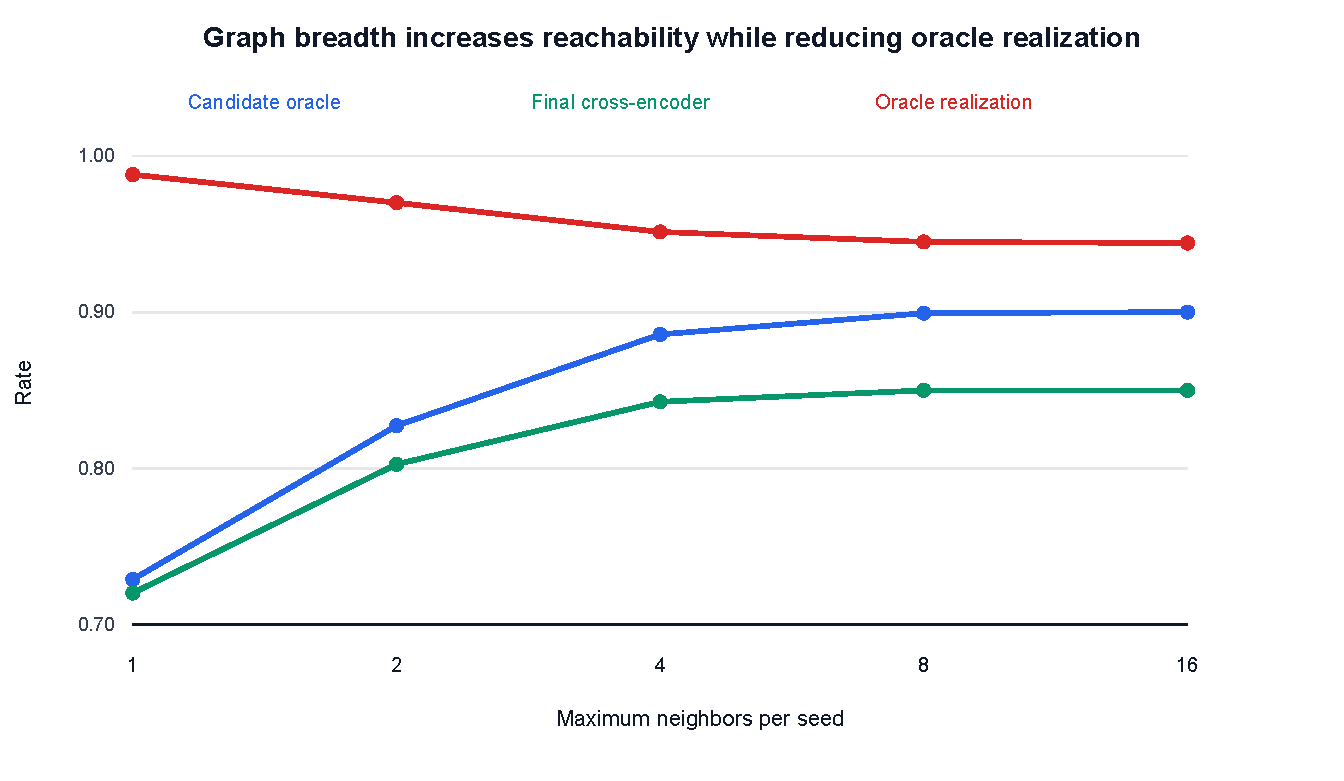
\includegraphics[width=\columnwidth]{figures/breadth-curve.pdf}
  \caption{Candidate reachability rises with graph breadth, but final recall
  saturates after eight neighbors per seed (MiniLM stack).}
  \label{fig:breadth}
\end{figure}

\subsection{RQ3: Citation expansion hurts LitSearch overall}

On LitSearch, citation pools lower BGE-reranked Recall@20 by 0.0369
[$-0.0681$, $-0.0066$] across all 597 queries. Both arms rerank equal-size
pools with the same reranker, and no edge scorer is used. The overall loss
hides a split by query source (Table~\ref{tab:litsearch}). Citation expansion
helps inline ACL queries, which describe cited papers, but hurts author-written
queries. For author-written queries the loss is mechanical. The citation pools
contain none of the 71 relevant papers that the seeds miss (0 of 49 for ACL
and 0 of 22 for ICLR), so the graph arm can only replace hybrid candidates with
non-relevant ones. For inline queries the pools contain 42 of 68 missed ACL
papers and 34 of 120 missed non-ACL papers. On inline
ACL queries, expansion also improves Complete@20 by 0.1327 and MRR@10 by
0.0407.

\begin{table}[t]
  \centering
  \caption{BGE-reranked LitSearch Recall@20 by query source. Over all 597
  queries the difference is $-0.0369$ [$-0.0681$, $-0.0066$].}
  \label{tab:litsearch}
  \small
  \begin{tabular}{lrrr}
    \toprule
    Query source & Hybrid & Graph & Difference \\
    \midrule
    ACL inline & 0.6320 & 0.7440 & \textbf{+0.1121} \\
    Non-ACL inline & 0.6976 & 0.6700 & -0.0277 \\
    Author ACL & 0.8000 & 0.6839 & \textbf{-0.1161} \\
    Author ICLR & 0.8462 & 0.7582 & \textbf{-0.0879} \\
    \bottomrule
  \end{tabular}
\end{table}

On MuSiQue, a scorer-ranked top 10 from the title-mention pool gains 0.0716
complete recall [0.0604, 0.0827] over the hybrid top 10, from 0.125 to 0.197.
This is not an equal-size pool comparison, because the graph ranking draws on
a larger pool. The scorer is trained on MuSiQue, so this is not a transfer of
the HotpotQA scorer, and the absolute level stays low. The BEIR tests use the
HotpotQA scorer without a cross-encoder. SciFact is neutral (0.0000 NDCG@10).
NFCorpus gains 0.0047 NDCG@10. Semantic
neighbors are useful boundary tests, but are not equivalent to hyperlinks or
citations.

\subsection{RQ4: Decomposition by gold reachability and degree}

\paragraph{Rescue coverage.}
On HotpotQA, rescue coverage correlates 0.731 with per-query document recall
gain across 7,405 queries (Table~\ref{tab:alignment}). Alignment features
explain 57.7\% of held-out variance, while bridge-versus-comparison labels
explain 3.8\%. This association is close to an identity. Rescue coverage
counts the missed gold documents that enter the graph pool, and the gain counts
gold documents that the reranked graph arm returns. Both read the same labels,
and the second is bounded by the first. The correlation shows that the BGE
reranker usually keeps reachable gold. It does not show that rescue coverage
predicts utility, and it cannot be computed at inference time. LitSearch shows
the same pattern (0.463 overall and 0.606 among queries whose seeds miss
evidence).

\begin{table}[t]
  \centering
  \caption{Five-fold ridge fits of per-query graph gain. Alignment features use
  gold judgments, so these fits are descriptive. Group uses coarse query
  labels.}
  \label{tab:alignment}
  \small
  \setlength{\tabcolsep}{4pt}
  \begin{tabular}{llrrrr}
    \toprule
    Corpus & Slice & $n$ & $r(A,\Delta)$ & Align. $R^2$ & Group $R^2$ \\
    \midrule
    Hotpot & All & 7,405 & .731 & .577 & .038 \\
    Hotpot & Missed & 2,187 & .633 & .403 & .043 \\
    LitSearch & All & 597 & .463 & .346 & .027 \\
    LitSearch & Missed & 239 & .606 & .334 & .103 \\
    \bottomrule
  \end{tabular}
\end{table}

The strata are also defined by gold labels. On HotpotQA, full-rescue queries
gain 0.3356 document recall over 1,813 queries, and no-rescue queries lose
0.1926 over 366. In the no-rescue stratum, the graph pool contains no missed
gold by definition, so graph recall equals seed recall (0.429). The deeper
hybrid pool reaches 0.622. The loss follows from the stratum definition. On
LitSearch, the corresponding differences are +0.4957 over 62 queries and
$-0.3441$ over 170. These contrasts describe the outcome. They are not a
discovered routing rule, because stratum membership is unknown before
relevance labels exist. The 5,218 HotpotQA queries whose seeds already hold all
gold change by 0.0011.

\paragraph{Target in-degree.}
On HotpotQA, standardized rescue among baseline misses is 0.034 for targets
with in-degree 0, 0.790 for in-degree 1, and 0.890 for in-degree 2 or more.
The highest-minus-lowest contrast is +0.8556 [0.8225, 0.8853]. Most of this
contrast is reachability. A target with no incoming link cannot be reached by
one-hop expansion from any seed, so its rescue must come from reranking
changes. The step from in-degree 0 to 1 is 0.756. The step from 1 to 2 or more
is 0.099. Their marginal intervals ([0.748, 0.832] and [0.870, 0.909]) do not
overlap, but I did not compute a paired interval for that step. The
degree-specific finding beyond reachability is therefore small. Degree is also
confounded with gold status, because validation gold paragraphs receive
31.5\% of all edges.

On LitSearch, the contrast between the highest bin (in-degree 5 or more) and
in-degree 0 depends on the standardization (Table~\ref{tab:litdegree}). With
query source in the strata, only 33 of 221 baseline misses fall in common
support, all from one query source, and the contrast is 0.000. Without query
source, 96 misses remain and the contrast is +0.1611. Query source is a known
effect modifier (Table~\ref{tab:litsearch}), so the second specification
leaves a known confounder uncontrolled. The first controls it but keeps little
data. Neither specification supports a reliable degree effect on LitSearch.
The two corpora also use different degree bins, so magnitudes are not
comparable.

\begin{table}[t]
  \centering
  \caption{LitSearch adjusted rescue contrast, highest minus lowest in-degree
  bin, among baseline misses. Both specifications also stratify by gold count.}
  \label{tab:litdegree}
  \small
  \setlength{\tabcolsep}{3pt}
  \begin{tabular}{lrr}
    \toprule
    Strata & Support & Contrast [95\% CI] \\
    \midrule
    Quality, specificity, source & 33/221 & 0.000 [$-0.352$, 0.267] \\
    Quality, specificity & 96/221 & +0.161 [0.025, 0.293] \\
    \bottomrule
  \end{tabular}
\end{table}

\subsection{Graph fusion has competitive risk}

Ordinary fusion can displace a parent result, so zero harm is the wrong
comparison. Here the HotpotQA and MuSiQue graph arms use the learned edge
scorer without a cross-encoder. Under the same best-parent definition, graph RRF has lower
document-recall harm than ordinary RRF on HotpotQA and MuSiQue and is tied on
LitSearch (Table~\ref{tab:fusionrisk}). Relative to the fixed hybrid baseline,
graph RRF improves versus harms 1,260/61 HotpotQA queries, 245/78 MuSiQue
queries, and 33/21 LitSearch queries.

\begin{table}[t]
  \centering
  \caption{Document-recall harm against the per-query best parent. Difference
  is graph minus ordinary RRF in percentage points.}
  \label{tab:fusionrisk}
  \small
  \setlength{\tabcolsep}{4pt}
  \begin{tabular}{lrrrr}
    \toprule
    Corpus & $k$ & Ordinary & Graph & Difference \\
    \midrule
    HotpotQA & 10 & 8.56\% & \textbf{4.39\%} & -4.17 [-4.97, -3.40] \\
    MuSiQue & 10 & 11.75\% & \textbf{9.64\%} & -2.11 [-3.85, -0.37] \\
    LitSearch & 20 & 6.20\% & 5.03\% & -1.17 [-3.85, 1.51] \\
    \bottomrule
  \end{tabular}
\end{table}

Depth is the main boundary. HotpotQA graph RRF stays below ordinary RRF harm
through cutoff 100 only when short graph lists are backfilled from hybrid.
Without backfill it has higher harm at cutoff 50 (3.35\% versus 2.85\%) and
100 (3.85\% versus 2.12\%).
MuSiQue is safer at 5 and 10, then reverses as title-mention candidates displace
stronger long-tail hybrid results. MuSiQue MRR and NDCG also remain weaker.
The evidence supports graph retrieval as a shallow fusion arm, not unbounded
traversal.

\subsection{Safety, scale, and downstream effects}

A fixed-$k$ sentinel reranks one baseline challenger with the graph shortlist.
On MuSiQue it reranks with BGE.
It improves 11 HotpotQA queries without harm, but on transfer it improves 13
MuSiQue queries and harms two. Appending that challenger changes the MuSiQue
count to 13/0 and returns at most $k+1$ documents. Preserving both result sets
requires their union and more output capacity.

The scale test is weaker than the main experiment. It uses MiniLM with no
cross-encoder and 400 questions from an internal split of the HotpotQA
validation set, not the full 7,405. The corpus has two million documents: the
66,576 validation-context paragraphs plus 1,933,424 added Wikipedia
paragraphs. The graph ranking orders the one-hop pool with the learned edge
scorer, frozen from a MiniLM run on the 141K-document corpus. At two million documents, the scorer-ranked graph top 10
reaches 0.6825 complete recall against 0.4550 for the hybrid top 10, a gain of
+0.2275 [0.1850, 0.2725]. Pool size is not controlled here, because the graph
ranking draws on a larger pool than the hybrid top 10. Absolute recall falls
as distractors grow.

On 1,000 HotpotQA questions, Qwen2.5-7B \citep{qwen2025qwen25} receives the top ten
documents from the BGE-reranked hybrid and hyperlink pools. Graph evidence raises complete recall from 0.805
to 0.929, exact match from 0.505 to 0.530, and token F1 from 0.6240 to 0.6643.
Answer changes follow evidence changes: graph wins when only graph retrieval
finds complete evidence, and loses when only hybrid does.

The tested no-op policies do not solve routing. Both gates use the MiniLM
scorer stack, not the BGE pools. A question-type gate, whose graph arm raises
complete recall from 0.590 to 0.820, mostly learns lexical cues. A local gate
whose features include overlaps with the scorer rankings can skip 4.51\% of
queries without a detectable recall loss, but a 12.11\% skip rate degrades
recall. A sweep of 25 two-hop Personalized PageRank policies in my engine also
fails to beat one-hop candidate recall at the same candidate count. That
sweep compares candidate recall only, not reranked results.

\section{Discussion}

The results read best as a negative result with one replication. On HotpotQA,
one-hop hyperlink pools recover the second gold paragraph of bridge questions
because the benchmark builds those questions from hyperlinks
\citep{yang2018hotpotqa}. That replicates the direction of earlier hyperlink
retrievers \citep{asai2020paths} on a smaller corpus and under a fixed budget.
Where questions are not built from the graph, the evidence is negative. Graph
pools do not help HotpotQA comparison questions, and citation pools lower
LitSearch Recall@20 overall and on author-written queries. This agrees with
\citet{singh2026beyond}, who find no reliable gain from graph expansion once a
strong reranker is present. My MiniLM GAR run also shows that reaching more
candidates does not guarantee a stronger final top-$k$ list.

The two decompositions say less than their large numbers suggest. Rescue
coverage and gain share gold labels. The in-degree contrast mostly restates
that one-hop expansion cannot reach unlinked targets. Neither gives a gate that
works before relevance labels exist. Like selective query expansion
\citep{cronentownsend2004selective}, the open problem is an observable signal
that predicts harm, and my routing experiments did not find one.

This study does not justify a default expansion policy. A graph should be
tested against the target query distribution, and a gain on a benchmark whose
questions come from the same graph is weak evidence for other workloads.

\section{Limitations}

\paragraph{Corpus.}
The HotpotQA corpus is a closed 141,232-document distractor set with 1.71
in-corpus links per document. Every gold paragraph is present, and the
distractors come from the same questions. Every bridge question's gold pair is
hyperlinked, and validation gold receives 31.5\% of the edges. The HotpotQA
gain is therefore largely a property of the benchmark's construction. Gains on
full Wikipedia may be smaller or larger. Citation-context queries can similarly
inherit citation alignment. LitSearch author-written queries and MuSiQue test
this concern only in part, and the random-edge control is too weak to test it.

\paragraph{Baselines.}
I ran no multi-hop retriever baseline, such as MDR \citep{xiong2021mdr},
HippoRAG \citep{gutierrez2024hipporag}, or the path retriever of
\citet{asai2020paths}. GAR was run only with MiniLM. Dense feedback is a simple
control, not the full class of iterative methods. The random-edge control
draws uniform targets and falls below its own hybrid pool, so it does not
isolate the value of authentic edges. A degree-matched or topic-matched
rewiring would be a stronger control. The strong stack covers one
encoder and one reranker.

\paragraph{Diagnostics.}
Rescue coverage, the rescue strata, and the alignment fits all use gold labels.
The degree audit uses the main experiment's own BGE rankings, so it describes
those rankings and not other rankers. Its associations are observational.

\paragraph{Multiplicity.}
I report many slices: question types, four LitSearch query sources,
alignment strata, degree bins, three fusion corpora, and a depth sweep. All
intervals are per comparison and unadjusted. The LitSearch degree contrast also
depends on the choice of standardization variables (Table~\ref{tab:litdegree}). Single-slice results,
especially on LitSearch, should be read as exploratory.

\paragraph{Scale and cost.}
The two-million-document test uses a weaker stack and 400 internal-split
questions. It adds controlled distractors rather than measuring online graph
maintenance or production tail latency. Append-only safety preserves set recall
by increasing output size. It does not guarantee better generation.

\section{Conclusion}

On the 141K-document HotpotQA distractor corpus, where every bridge question's
gold pair is hyperlinked by construction, one-hop expansion reranked by BGE
raises complete recall from 0.784 to 0.934 against an equal-size hybrid pool.
On LitSearch, citation expansion hurts overall and on author-written queries,
and helps only inline ACL queries. Rescue and degree diagnostics are
descriptive. Graph expansion helped here where the benchmark was built from the
graph, and did not help elsewhere.

\bibliographystyle{abbrvnat}
\footnotesize
\setlength{\bibsep}{1.5pt plus 0.3ex}
\bibliography{references}

\end{document}
